\documentclass[version=last,fontsize=13pt]{scrartcl}


\usepackage{pdfpages}
\usepackage{graphicx}
\usepackage{indentfirst}

\usepackage{titlesec}
\usepackage{caption}

\titlespacing*{\section}{0pt}{3ex}{3ex}
\titlespacing*{\subsection}{0pt}{1.5ex}{1.5ex}
\titlespacing*{\subsubsection}{0pt}{1.5ex}{1.5ex}

\usepackage[margin = 0.8in]{geometry}

%my own paragraph for which the text that follows starts on a new line
\newcommand{\myparagraph}[1]{\paragraph{#1}\mbox{}\\}

% dont number sections
\setcounter{secnumdepth}{0}

\usepackage{wrapfig}
\usepackage{float}

\usepackage{caption}
\usepackage{subcaption}

\usepackage{tabularx}
\begin{document}

\begin{titlepage}
	\begin{center}	
		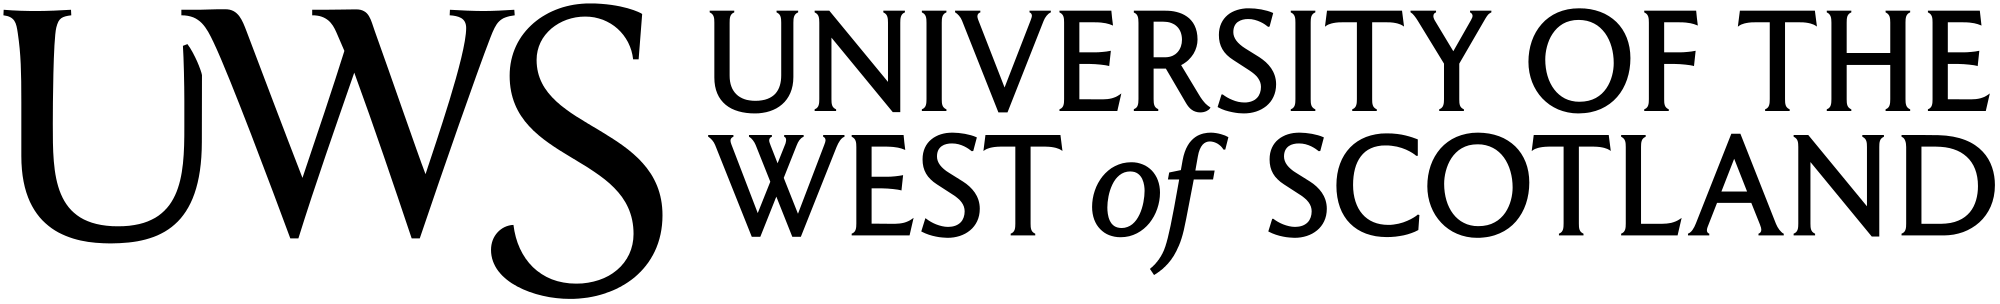
\includegraphics[width = 5cm,height = 1.5cm]{./imgs/uws_logo.png}\\[5cm]
	
	 { \huge \bfseries %
		How can Android Packed malware be detected and prevented?\\} 

	\vspace{6cm}			
			
		\begin{flushright}
				\large Student:\\
				Marius-Lucian Olariu\\[1cm]
		\end{flushright}
		
	
		\begin{flushleft}
			 \large
				Supervisor: \\
				Dr. Zeeshan Pervez \\[1cm]
		\end{flushleft}
		
	\vspace{2cm}	
	
		
		\vfill

			{\large {Paisley \\ 2019}}
		\end{center}
\end{titlepage}

\renewcommand{\labelenumi}{\roman{enumi}}

\newpage

\tableofcontents

\newpage

\listoffigures


\newpage


\section{Introduction} 


%add information from the presentation slides and speakers notes

%summarise the traditional packaging technique
	Android is an \textbf{O}perating \textbf{S}ystem (OS) designed for mobile devices like tablets and smartphones and is currently the market leader  of mobile operating systems since  2016 (Mobile OS Market Share 2018, 2019). Android has been the leading mobile OS in phones sold since 2011 as can be seen in Figure~\ref{aStats} (Mobile OS Market Share 2018, 2019). The CEO of Google, Sundar Pichai, declared at Google I/O 2017 that there are over two billion smartphones running Android OS  (Google I/O 2017, n.d). The success of Android is due to the fact that is very efficient (uses a modified version of the Linux kernel) and open-source.  The fact that Android is open-source and has a large number of users it  attracts a lot of attackers to develop malware (at stake is huge material gain and prestige). The problem of Android malware is similar to the one Windows OS faces, in other words, because most of the personal computers run Windows most of the  malware targets Windows systems and not Linux or macOS systems. Another fact that makes Android so appealing to malware authors is the possibility to install \textbf{app}lication\textbf{s} (apps) from unknown sources and  there are many third-party markets where one can get such apps.\\ 

	\begin{figure}[H]

		\caption{Global market share sales by mobile OSs from 2009 to 2018}
		\label{aStats}

		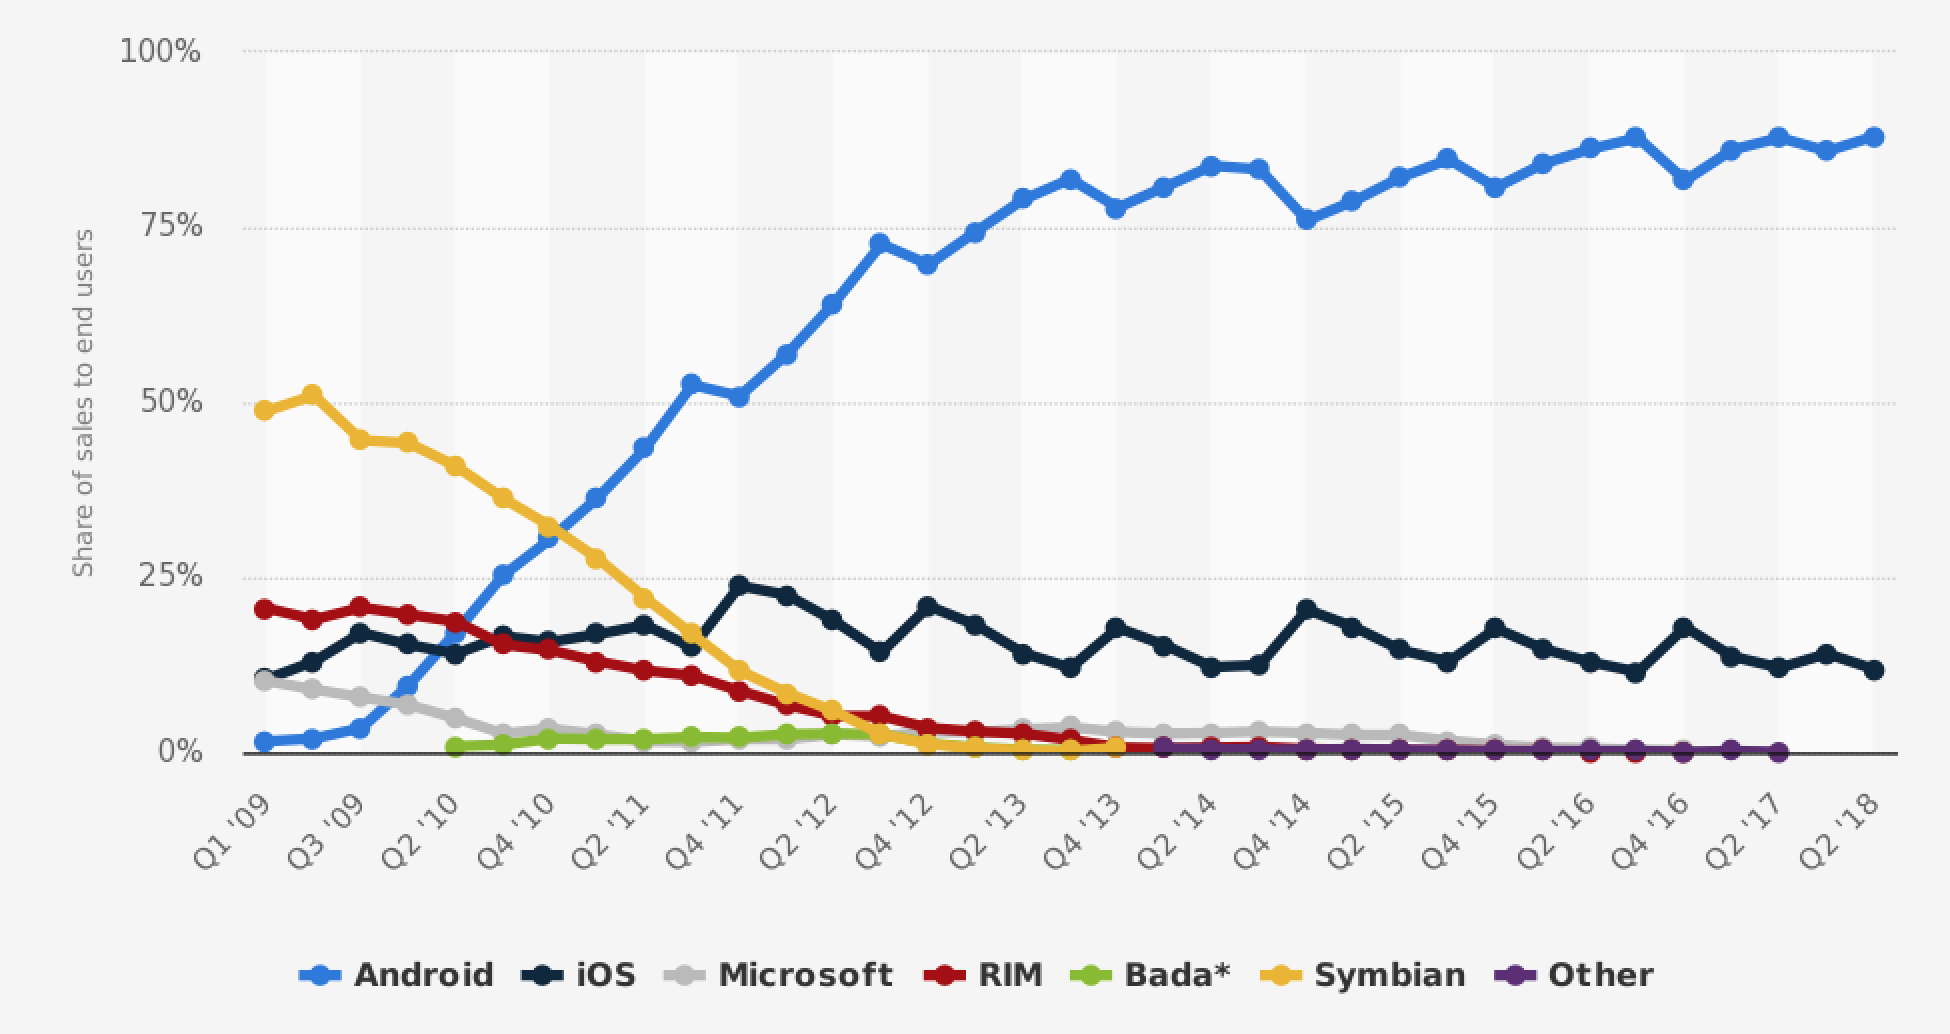
\includegraphics[scale = 0.48]{./imgs/androidStats.png}
	\end{figure}
	
	\indent
	Android apps are distributed and installed using the \textbf{A}ndroid \textbf{P}ac\textbf{k}age (.apk) format. The apk format is essentially an archive (was extended from JAR and ZIP) that contains the \textbf{app}lication (app) compiled code, resources, certificates and the manifest file. Because an apk file it is just an archive it can be easily unarchived, thus it a fairly straightforward process to get to the compiled code of a certain app once you have the apk file. For Android the compiled code is in \textbf{D}alvik \textbf{Ex}ecutable (DEX) format and because executable code is hard to understand for a human it needs to be further converted. DEX code can be converted to a human-readable code known as \textit{smali} using open-source tools like \textit{Apktool} (Tumbleson, n.d.). Moreover, \textit{Apktool} recovers the xml files and Android manifest file to a form close to the original ones. Typically, a smali file contains the compiled code of a Java class. In order to add malicious code the attacker can add smali code in the app files or add new smali files containg malicious code. For instance one could write a broadcast receiver that reads and sends the phone contacts of the users to a webserver and is triggered when the user restarts his phone, this does not need too much effort from an attacker. Once the malicious code is added to the app, the attacker repackages everything  into an apk file (representing the malicious Android app). The next step is to sign the newly created apk file which can be done either using a certificate authority or a private key generated by the attacker of the app, obviously the attacker will pick the later variant. The signing of an apk file should help Google identify the author of an app, however, non-official markets are not really interested in finding the authentic author of an app. At this point the attacker has "cloned" a genuine app and is free to redistribute it (Crussellm Gibler and Chen, 2012) .  In short,  the above-described process is known as the \textit{repackaging attack}, please see Figure~\ref{repA} for a visual depiction of the attack (Wenliang, 2015) .\\

	\begin{figure}[H]
		\centering
		\caption{Overview of the repackaging attack}
		\label{repA}

		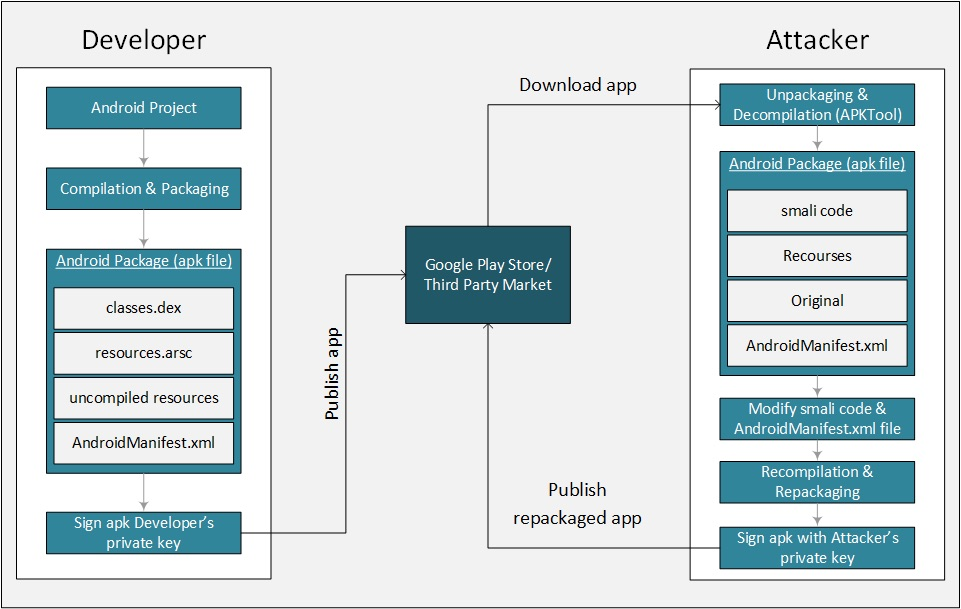
\includegraphics[scale = 0.50]{./imgs/repackAttack}
	\end{figure}
	
	
	\indent
	In order to protect from the repackaging attack there have been developed Android Packers that can enhance Android apps by providing anti-decompliation, anti-runtime injection and anti-debug techniques. The Android Packers are available only through web portals where the developer can upload his apk file and get it in the \textit{packed} format which is safer for distribution on app markets.  However, recently the Android Packers have started to be used not only by developers to protect their intellectual property but also by hackers to better hide malware in apps (Yang et al, 2015).  A packed app  poses a real challenge for security specialists because it is really hard to be analyse to detect if is benign or malicious.  


\section{Literature review}

\subsection{DroidUnpack}
	DroidUnpack is a framework developed for detection and analysis of Android apps with packed malware and it can monitor app execution at the lowest level and also reconstruct Java level execution (Duan et al., 2018). In other words, DroidUnpack is an emulator that can run the Android OS with the app to be analysed and monitors the memory writes performed by the app. The framework has been tested against 93 910 Android apps containing malware (13 556 containing packed malware), 6 major commercial packers (Ali, Baidu, Bangle, Ijiami, Qihoo and Tencent) and 3 unpackers (DexHunter, AppSpear and Kisskiss) over a large time frame (2010 - 2015) and the authors want to make it public in the future.\\
	DroidUnpack makes use of the following tools to investigate a packed app:

	\begin{enumerate}
		\item  JNI inspector
		\item  Hidden Code Extractor
		\item  Multi-layer Unpacking Detector
		\item  Self-Modifying Code Detector
	\end{enumerate}

   	\indent
	When developing an Android app the developer can use multiple languages like Java, C++ and C. The \textbf{J}ava \textbf{N}ative \textbf{I}nterface (JNI) is a framework that enables communication between code written in Java and code written in C/C++ (which is put in libraries referred to as \textit{native libraries}). Attackers can avoid static analysis detection of Android API sensitive calls by creating recursive calls between methods written in C++ and methods written in Java thus JNI inspector tool tries to track the whole sequence of method calls.\\
	\indent
	The Hidden Code Extractor feature extracts hidden packed executable at runtime by making use of the \textit{program counter} (pc) and interceptions of every memory write.\\
	\indent
	The Multi-Layer Unpacking tool looks for code that is continuously decrypted but not executed and only when the execution takes place  is considered the end of a layer, this tool also inspects the memory writes.\\
	\indent
	Once an executable is launched it is possible to modify its code and this is known as \textit{self-modifying code}. For example, on Android one can call native code using JNI that in turn can access memory locations storing DEX bytecode and modify them. Moreover, using the same procedure even data structures used by DEX bytecode can be modified in memory, thus self-modifying code is indeed a powerful practice. The Self-Modifying Code Detector tool finds self-modifying code by searching for patterns like \textit{execute - write - execute} on the same memory location.\\
	\indent
	If an app requires multiple processes to be run (very unlikely for a benign app) the framework can detect when a \textit{fork} takes place and can link a new process to the parent process from which it was created. This behaviour is achieved by modifying the \textit{libcutils.so} native library and is very useful in order to understand what an app does under the hood.\\
	\indent
	DroidUnpack supports only Android 4.2 and 5.0 at the moment which is a drawback, in my opinion, considering that the current version of Android is 9.0 and there are not that many devices on the market that still run Android 4.2/5.0. However, the authors of the framework say that DroidUnpack can be easily tweaked to support other Android versions. Another shortcoming of DroidUnpack is the fact that it cannot analyze apps that have anti-emulation detection (i.e. the apps that can detect that they are running on an emulator; if so, they can modify their behaviour). The problem with apps that have anti-emulation in place is faced by the vetting process of Google Store as well.  Google also runs the apps on an emulator for a specific time amount (e.g. 24h) to analyse their behaviour  but an attacker could code the app to launch  an attack only after the app has been used for more than one week let us say. 
	For a general view of the DroidUnpack framework please see Figure~\ref{droid} (Duan et al., 2018).


	\begin{figure}[H]
		\centering
		\caption{Overview of the DroidUnpack framework}
		\label{droid}

		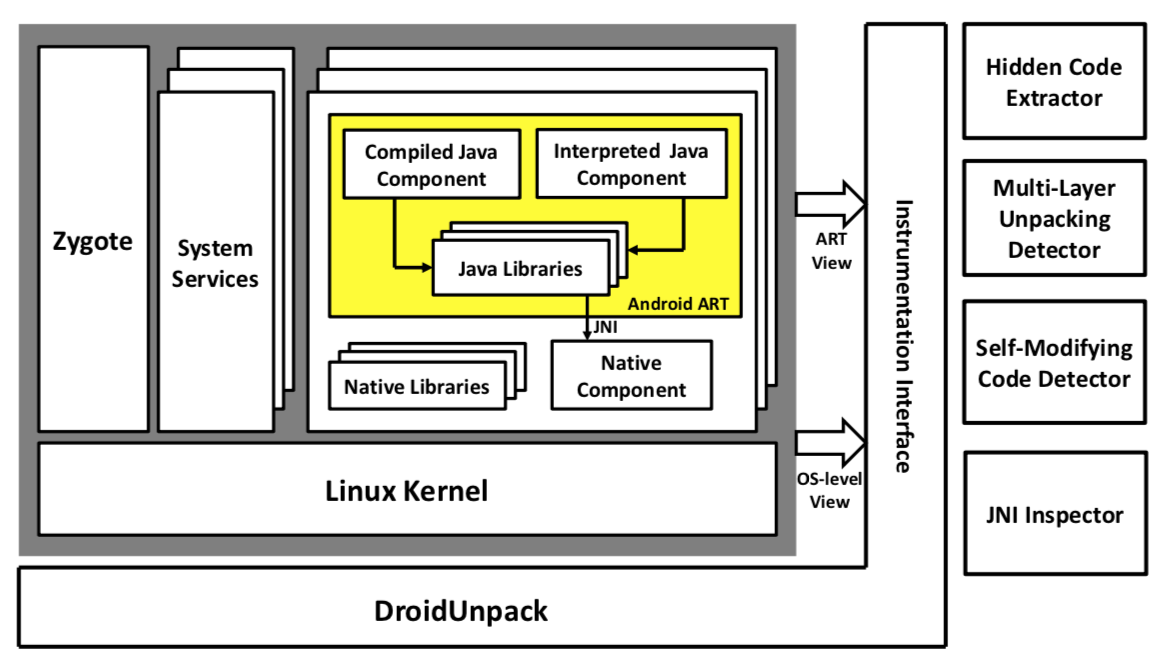
\includegraphics[scale = 0.8]{./imgs/droidUnpack}
	\end{figure}
	
\subsection{DexHunter}
	One important step in finding if a packed app contains  malware is to do a static analysis of the source code of the app. However, a packed app has anti-decompilation protection so it is not easy to get to the DEX code. DexHunter is a software system that can extract the DEX files of  packed apps, also known as unpacker software (Zhang, Luo and Yin, 2015). Starting with Android 4.4 the runtime \textbf{D}alvik \textbf{V}irtual \textbf{M}achine (DVM) was replaced with \textbf{A}ndroid \textbf{R}un\textbf{t}ime (ART), nonetheless, DroidHunter works with both runtimes. The unpacker was tested on apps that were packed with six major packers (Bangle, Tencent, 360 Mobile, Ijiami, Ali and Baidu).\\
	\indent
	In order to get to the unpacked DEX bytecode DexHunter works on a physical device when the app to be analysed is running and locates the memory region where the app is loaded and dumps it. Two approaches have been devised for the two different Android runtimes, DVM and ART. However, in order to obtain the DEX bytecode the authors of DexHunter have modified the DVM and ART runtime on the physical phones where DexHunter was run. Every packer introduces some kind of overhead to the packed app, it could be extra files, new classes or a modified \textit{AndroidManifest.xml}. The authors of DexHunter profiled what files each studied packer introduces so that DexHunter can determine with which packer an app was packed. For apps that are potentially packed with unknown packers (not the 6 ones mentioned above), DexHunter looks for dynamic code modification and if that happens it regards an app as being packed.
	In the Figure~\ref{dexHunt} (Zhang, Luo and Yin, 2015) it can be seen an overview of the whole process that DexHunter uses to get the DEX files of a packed app.

	\begin{figure}[H]
		\centering
		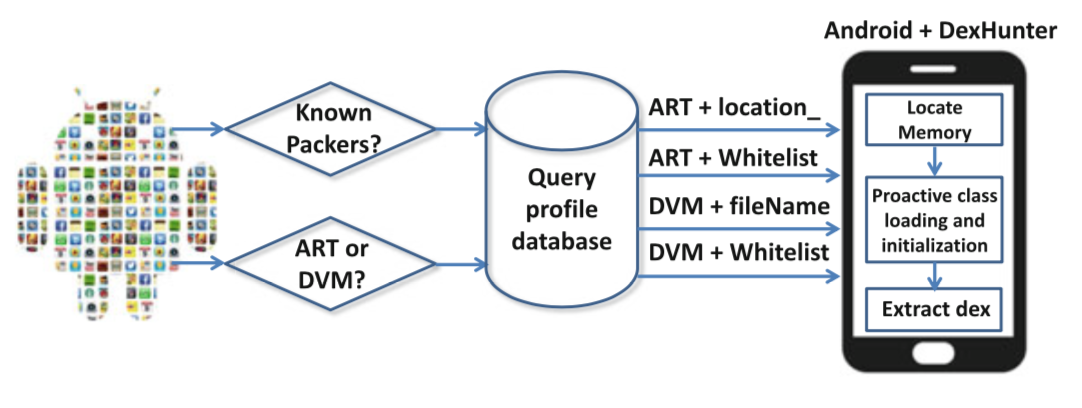
\includegraphics[scale = 0.8]{./imgs/dexHunterFlow}
		\caption{Using DexHunter in smartphone to recover DEX files from packed apps}
		\label{dexHunt}
	\end{figure}

	The evaluation of the DexHunter was done by running it against 40 apps downloaded from F-Droid market which were packed by the authors using the 6 packers mentioned above. However, not all 40  apps could be packed and some of them were not running after being packed. It was found that the packed apps are in general larger and have a prolonged launch time than the original ones. DexHunter managed to recover the DEX files for apps packed with Ijiami, 360 Mobile, Baidu and Bangle packer in both ART and DVM; for Bangle the dumped DEX files were incomplete. Ali packer only works packs apps for DVM runtime and DexHunter managed to get the DEX files for apps packed with Ali packer. DexHunter was not able to recover the DEX files of the apps packed with Tencent.

\newpage

\section{Security and privacy advancement and glitches} 
	In the following lines, the authors is going to summarise what can be gained by an attacker by doing the repackaging attack.

\myparagraph{Advertisement}
	\indent
	One of the main incentives for cloning an app is for material gain, thus, an attacker normally picks apps that are popular on Google Store and gets their apk (Gibler et al., 2013). Each published app contains a developer id which is used to direct advertisement revenue to the developer and can be changed. The attacker changes the developer id to himself, repackages the app and publishes it on another market and the advertisement revenue goes to the attacker. Another way of redirecting the advertisement revenue is to change the advertisement libraries used by the app.

\myparagraph{API key}
	\indent
	Most of the cloud services available to Android apps use a key to identify the traffic generated by an app and charge the developer accordingly. Often beginner developers or developers who are not aware that their app can be reverse engineered just store their API keys as constants in app source code. It is obvious that once the API key gets into the hands of the attacker he can use it in his own apps without being charged for the used services. It is very hard for the developers to find out that their API key is compromised.

\myparagraph{App cracking}
	\indent
	One way to generate revenue is to provide a limited access to some of the app features and for others, the developer can require the user to pay to get a 'pro' version. Once the app is decompiled the attacker can identify where the check to see if the user has paid for the pro variant is done, take it out, repackage the app and distribute it on third-party markets. 

\myparagraph{Credential sniffing}
	\indent
	In order to provide personalized content to a user many apps use a login mechanism. Once the app is decompiled the attacker can change  the authentification mechanism and steal the login credentials of the users when they try to login.

\myparagraph{Financial fraud}
\indent
	Many Android games today are played by the young generation and due to their competitive nature some of them provide different in-app purchases to enhance the gameplay experience. A repackaged app can circumvent the need for payment for in-app purchases thus it will lure users to download and use it. Once the app is downloaded the attacker can ask for additional permissions non-related to the app and steal sensitive information (Ruiz, 2016). Another possibility is to direct the revenue for the in-app purchases from the developer to the attacker.

\myparagraph{Man-in-the middle attacks}
\indent
	If not through the direct methods mentioned above like advertisement and financial fraud an attacker can still generate revenue by tracking users actions within the app. Nowadays, data about  users is valuable because it can be analyzed on a large scale using big data algorithms and the attacker can sell it. In the end, the user will see fine-tuned advertisement based on his online behaviour.\\

\indent
	The consequences of app repackaging attack from the developer perspective are the following.

\myparagraph{Loss of intelectual property}
\indent
	Whether the development of an app is done in order to gain revenue out of it or just for fun the loss of one's work is daunting. Unfortunately, it is very hard to trace the attacker and to make him accountable for his actions.

\myparagraph{Customer loss}
\indent
	Nowadays, news travel fast and people use online forums to share information regarding apps. Once it is found that an app has been compromised the customers will look for alternatives that provide the same functionality.

\myparagraph{Reputational loss}
\indent
	If one of the apps from a certain company/developer gets reverse engineered and is found, all the other apps developed suffer. It does not matter that the other apps are secure because people will not trust the developer/company anymore.

\myparagraph{Fines for data breaches}
\indent
	If a certain app works with customer data like names, credit cards or home address it is exposed to the \textit{credential harvesting} mentioned above. The app developer can be directly prosecuted for a data breach, for instance, the average fine for a data breach in 2018 in UK was aroung £ 150 000 (Breavington, 2018).

\myparagraph{Incident handling cost}
\indent
	Even if the app developer finds out that his app has been plagiarized and published on a third-party market it might take a significant amount of time to get it down (not always possible).
	
\myparagraph{Investor distrust}
\indent
	If one of the apps for which a developer was founded gets cracked the investor will not work with that developer again, also the news about this will spread in investor's business network.

\pagebreak
\section{Real-world scenarios, use cases}
%examples to demonstrate the impact
%talk about Obfuscated Malware discovered on google Play

\subsection{ExpensiveWall}
	ExpensiveWall is a malware family that subscribes users to fake services which use premium SMS messages to gain revenue and is essentially a trojan (ExpensiveWall: A Dangerous 'Packed' Malware On Google Play, n.d.). Google confirmed that about 50 apps were infected with this type of trojan and they were downloaded in total between 1 million and 4.2 million times before being removed from Google Store in 2017. However, this did not solve the problem completely since the apps remained installed on users devices, Google did not use their "kill switch" to remove them from devices as they did for DroidDream (n.d.). Apps that contained ExpensiveWall were packed.\\
	\indent
	One of the apps that contained ExpensiveWall trojan was 'Lovely Wallpapers' which provided users with photos for their phone home-screen. However, apart from requiring Internet access permission (which is understandable) it also asked for SMS permissions (which nowadays are labeled by Google with protection level "dangerous"). SMS permission allowed the app to send premium messages. The difference between  app functionality and the SMS permissions it asked for should have been obvious to a cautious user. Starting with Android 6.0 the user is no longer required to grant all app permissions before installing the app; the app permission are required individually when they are  needed, nonetheless, still more than 1 million users were tricked. The first step "Lovely Wallpaper" was doing after app installation was to send user location, device identifiers, MAC and IP addresses to a webserver controlled by the attacker. Next, whenever user's device connected to the Internet a webpage containing links  to premium SMS services was sent to the app. The app then silently clicked on those links and the user got subscribed to the SMS services. In other cases, the user was asked to press on a "Continue" button which would trigger the sending of a premium SMS through a simple webpage containing JavaScript code (see Figure~\ref{simpleJS}).\\
	
	\begin{figure}[H]
		\centering
		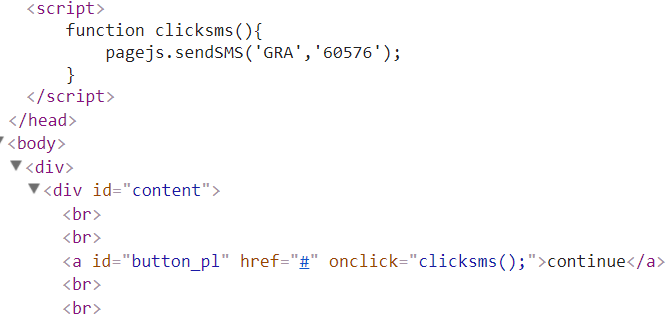
\includegraphics[scale = 0.60]{./imgs/simpleJS.png}
		\caption{Web code snippet for sending a premium SMS in "Lovely Wallpaper" app}
		\label{simpleJS}
	\end{figure}

\subsection{ValerySoftware}
	One good sector for repacking apps is gaming because a big part of the users are young people who tend to be more naive when installing new apps. A series of packed apps containing malware were published by a developer known as "ValerySoftware" (see Figure~\ref{vS}). The apps were targetting the famous Minecraft  game and they were detected on Google Store on 2016 by a McAfee security researcher (Ruiz, 2016). However, this time the consequences were not so big because only around 3000 devices were infected. All the apps shared some common behaviour like having code  obfuscated multiple times, anti-emulation detection, advertisement clicking or leaking sensitive user information. Code obfuscation and anti-emulation (hampers debugging on emulators) are known features provided by app packing technique.\\

	\begin{figure}[H]
		\centering
		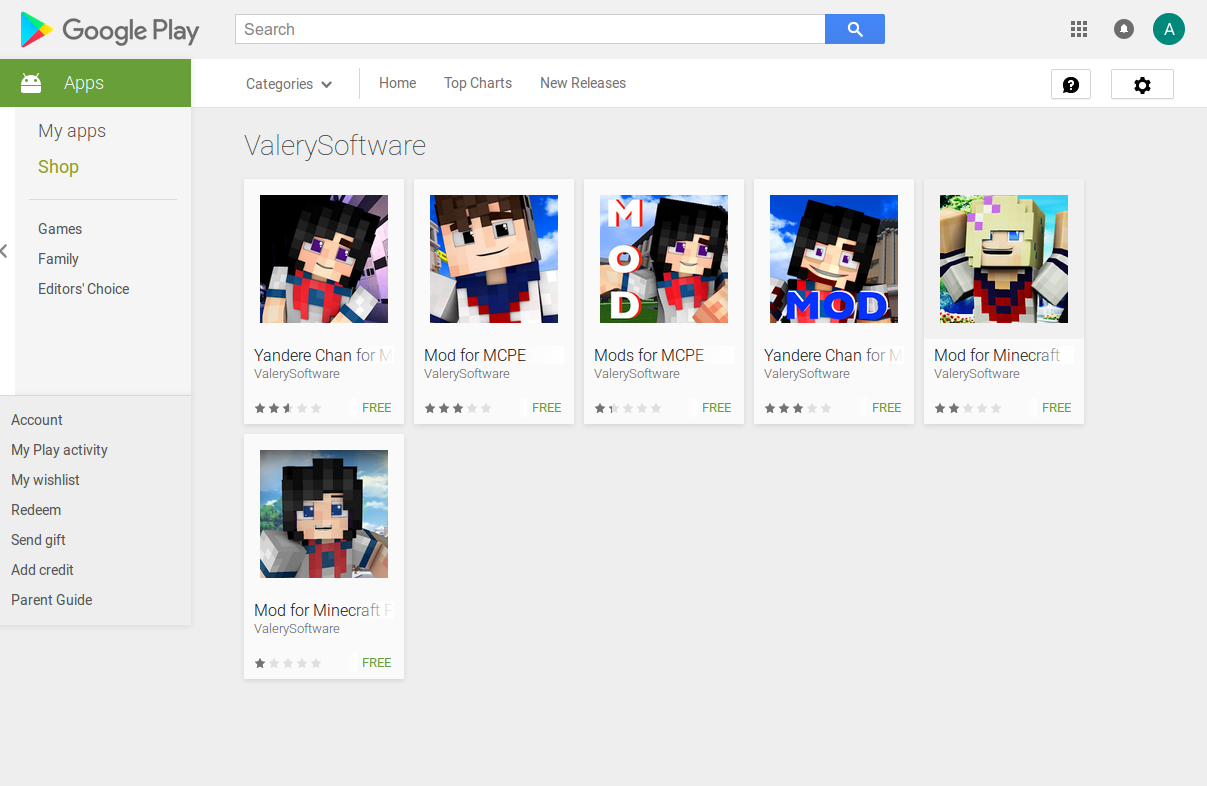
\includegraphics[scale = 0.65]{./imgs/valerySoft.png}
		\caption{Packed applications containing malware published by ValerySoftware}
		\label{vS}
	\end{figure}

	\indent
	In general, the apps did not provide functionalities, a fact signaled by users on Google Store forum.  Under the hood, they decrypted packed malware stored in the assets region of the apk file. Moreover, some malicious JavaScript and HTML code were encoded in DEX files (Android executable code) and loaded at runtime.\\
	\indent
	Google does a good job in protecting users from repackaged apps and responds promptly when they are signaled about an app containg malware. Most of the repackaged apps are published on third-party markets where the app vetting process is not so strict.

\section{Conclusion}
\indent
	Due to the fact that Android is the most popular mobile operating system attackers constantly try to create malware for it. The down-side of being open-source is the fact that everyone can study it in detail and this can cause security problems. One of the problems for the Android platform is that by default it does not enforce the developer to use binary protection methods before publishing the app. Due to this fact, the app published can be reverse engineered, modified and redistributed. To protect from apps from this vulnerability there have been devised Android packers that try to provide binary protection to an app (code obfuscation, anti-emulation, anti-runtime injection etc.). However, these packers have been aused by malware authors to protect cloned apps against malware detection. In order to understand how malware authors exploit packers, various solutions have been proposed in literature like DroidUnpack (framework for detecting packed malware) or DexHunter (software that can extract DEX code from a packed app). Recently, also the companies that provide packing services through web portals have started to first check the app that is going to be packed if is benign or not.\\
	\indent
	Once  an app is reverse engineered all kind of outcomes are possibles like advertisement hijacking, credential sniffing or API Keys stealing. We have seen that packed apps containing malware can circumvent even Google's official app market security mechanisms. In the first case, ExpensiveWall, a large number of users were affected while in the second, ValerySoftware, not so many because Google managed to take down the malicious apps shortly after they were published.\\
	\indent
	In my opinion, Google should modify the way Android apps are distributed and create a new packaging format that has binary protection. Google has enough resources to design a packaging format that is secure instead of leaving the developers with the burden of securing their app through various solutions like packers that are not so reliable as it was shown in this work. 
\pagebreak
\section{References}

Breavington, R. (2018) \underline{Average Fine For Data Breaches Doubles To £146,000 In}\\ \underline{Just A Year} [Online] Available: https://bit.ly/2Fwii8f [Accessed: 27 March 2019]\\

Crussell, J., Gibler, C. and Chen, H. (2012) \underline{Attack of the clones: Detecting cloned}\\ \underline{applications on android markets} In European Symposium on Research in Computer Security  Berlin : Springer\\

DroidDream. (n.d.) [Online] Available: https://bit.ly/2U1aljZ [Accessed: 27 March 2019].\\

Duan, Y., Zhang, M., Bhaskar, A.V., Yin, H., Pan, X., Li, T., Wang, X. and Wang, X. (2018) \underline{Things you may not know about android (un) packers: a systematic study}\\ \underline{ based on whole-system emulation} In 25th Annual Network and Distributed System Security Symposium  s.l. : NDSS \\

\underline{ExpensiveWall: A Dangerous 'Packed' Malware On Google Play} (n.d.) [Online] Available: https://bit.ly/2h55Q1K [Accessed: 27 March 2019]\\

\underline{F-Droid} (n.d.) [Online] Available: https://f-droid.org/en/ [Accessed: 26 March 2019]\\

Gibler, C., Stevens, R., Crussell, J., Chen, H., Zang, H. and Choi, H. (2013) \underline{Adrob: }\\ \underline{Examining the landscape and impact of android application plagiarism} In Proceeding of the 11th annual international conference on Mobile systems, applications, and services s.l : ACM\\

\underline{Google I/O 2017.} (n.d.) [Online] Available: https://bit.ly/2CvBOjd [Accessed: 12 March 2019].\\

\underline{Mobile OS Market Share 2018.} (2019) [Online] Available: https://bit.ly/2Fwii8f [Accessed: 24 March 2019].\\

Ruiz, F. (2016) \underline{Obfuscated Malware Discovered On Google Play} [Online]  Available: https://bit.ly/2UcWx5y [Accessed: 12 March 2019] \\

Shao, Y., Luo, X., Qian, C., Zhu, P. and Zhang, L. (2014) \underline{Towards a scalable}\\ \underline{resource-driven approach for detecting repackaged Android applications} In Proceedings of the 30th Annual Computer Security Applications Conference  s.l: ACM\\

Tumbleson, C. (n.d.) \underline{Apktool.} [Online] Available: https://ibotpeaches.github.io/Apktool/ [Accessed: 24 March 2019].\\

Wenliang, D. (2015) \underline{Android Repackaging Attack Lab} [Online]\\ Available: https://bit.ly/2urlfRa  [Accessed: 24 March 2019]\\

Yang, W., Zhang, Y., Li, J., Shu, J., Li, B., Hu, W. and Gu, D. (2015)\\ \underline{Appspear: Bytecode decrypting and dex reassembling for packed android malware}. In International Workshop on Recent Advances in Intrusion Detection (pp. 359-381) Cham: Springer \\

Zhang, Y., Luo, X. and Yin, H., (2015)  \underline{Dexhunter: toward extracting hidden code}\\ \underline{from packed android applications}  European Symposium on Research in Computer Security (pp. 293-311) Cham: Springer\\

\end{document}

